\chapter{运行时可定制调度的沙箱机制实现}\label{chap:control_zone}

\section{概述}

% 介绍 Control Zone 的概念
% - 面对什么场景
% - 存在哪些问题
%   - 复杂的硬件环境
%   - 复杂的软件环境
% - 针对每个问题的解决方式
% - 设计目标

数据中心的混部场景存在两个显著特征。在硬件上,现代服务器上拥有丰富的计算资源,能够支持大量的任务同时运行,同时硬件环境也相对复杂,混部时需要充分考虑硬件的特性,从而能够避免产生竞争。在软件上,数据中心上运行的应用种类十分丰富,同时不同应用对于不同的资源存在不同的需求,粗略地将应用分为LC与BE类型通常会忽略其他混部的可能,而根据其他竞争资源细分应用的类型,则需要有相应的调度机制来进行保障。

本研究提出了Control Zone,一种运行时可定制调度的沙箱机制实现。在航空领域,Control Zone指受控空域的一部分,通常在机场的周围,保护进出机场的的空中交通,而机场内,调度通常由塔台完成。本研究中借用此概念实现了如下特性:

1)容器运行时:Control Zone中包含有一个精简的容器运行时,支持运行丰富的容器应用,同时为避免重复的容器镜像开销,Control Zone相互共享只读层镜像。

2)轻量级虚拟机:Control Zone虚拟机包含了一个裁切后的最小化内核、精简的根文件系统、以及轻量级Hypervisor,这些手段减少了虚拟化环境的开销,同时也支持不同虚拟机实现来扩展更多的功能。

3)Sched Ext调度类:Control Zone内核支持Sched Ext调度类,BPF Scheduler以容器镜像的形式打包,并支持在运行时动态切换BPF Scheduler。

4)可观测系统:Control Zone包含了一个围绕虚拟机的可观测系统,能够从Host、Hypervisor、App三个不同的层次采集丰富的指标数据,用于监测Control Zone及其中运行应用的性能。

\begin{figure}[!htbp]
    \centering
    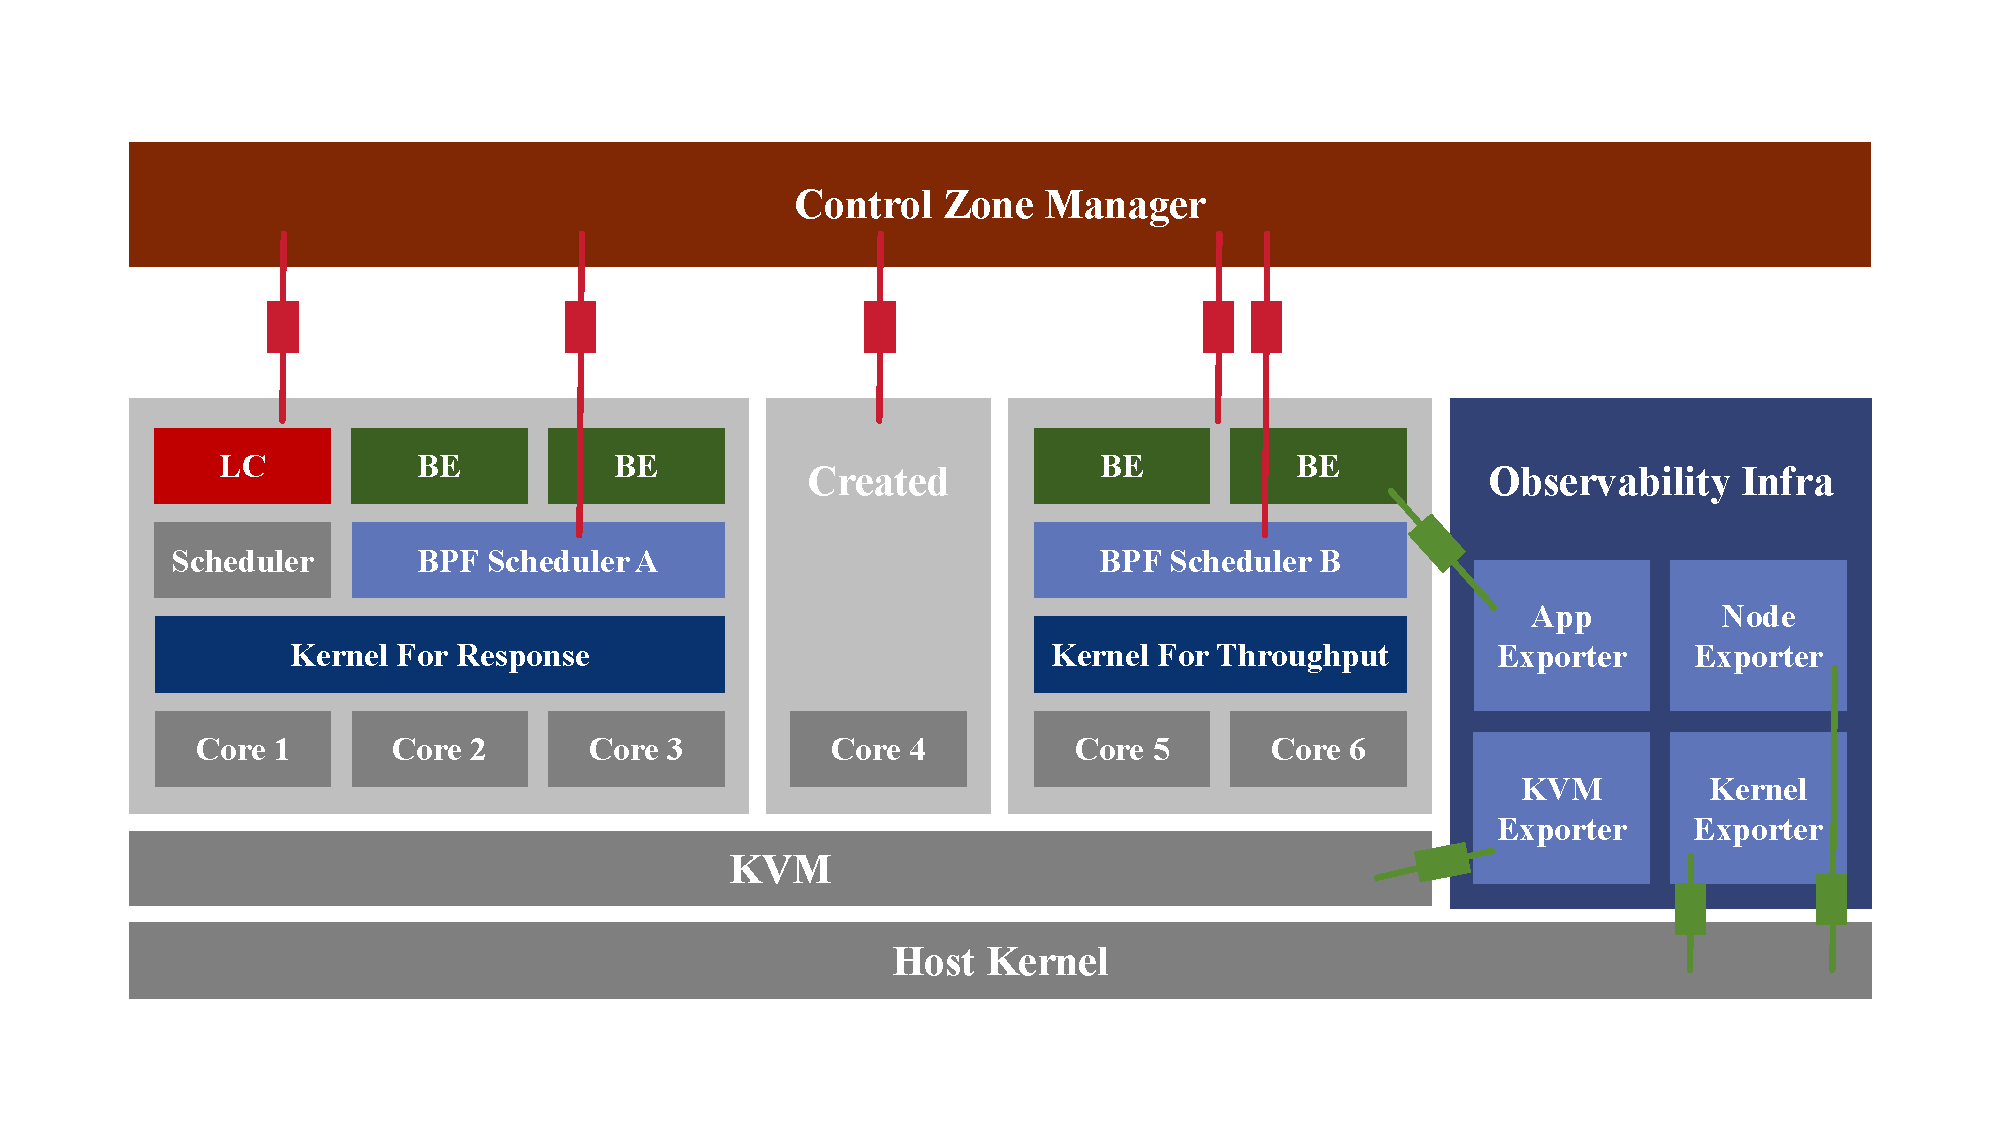
\includegraphics[width=1.0\textwidth]{controlzone_arch}
    \bicaption{\quad Control Zone基本架构}{\quad Control Zone Architectural}
    \label{fig:controlzone_arch}
\end{figure}
 
运行时可定制调度的沙箱机制通过如图~\ref{fig:controlzone_arch}所示分解数据中心单节点上的混部场景。首先,根据不同硬件资源特性将服务器分割为有限个Control Zone并进行标注,Control Zone之间允许最大程度的并发运行,而借助Hpyervisor及Host提供的隔离能力,严格限制不同Control Zone之间的资源边界。其次,根据不同的Control Zone的硬件资源特性选择匹配的精简内核,这样做一方面能够适配硬件的特性,另一方面去除掉冗余的代码,减少内核大小。随后,在启动任务时考虑应用的特征,分发应用到合适的Control Zone或启动一个ControlZone用来装载应用。而在Control Zone运行的整个过程中,可观测基础设施可以被选择性地激活,用来对Control Zone及其中的应用性能进行观测分析。最后,Control Zone中调度器容器作为塔台,可以根据调度目标以及硬件特性选择合适的定制调度机制,并在变化时进行动态修改,保障关键应用的性能。

\section{Control Zone组成}

% Control Zone组成,阐述各个组成部分所做的功能,希望实现的目标
% - czctrl: Control Zone管理
% - czdaemon: 容器管理
%   - chsd: 调度策略管理
% - observity: 可观测性

运行时可定制调度的沙箱包括Control Zone管理、应用管理及可观测性三个主要部分。如图~\ref{fig:cz_components}所示,用户通过czyaml配置文件来定义一个Control Zone,而Control Zone的管理主要czctrl、czmanager及虚拟化运行时三个组件协作完成。每个Control Zone都运行有一个czdaemon,并与czctrl、czmanager协作实现应用管理。可观测性沿用了第三章中设计的在线指标监测系统,通过与czmanager的协作完成对于虚拟机的监控。镜像存储服务负责管理OCI镜像,并在Control Zone管理的各个阶段提供镜像存储服务。

\begin{figure}[!htbp]
    \centering
    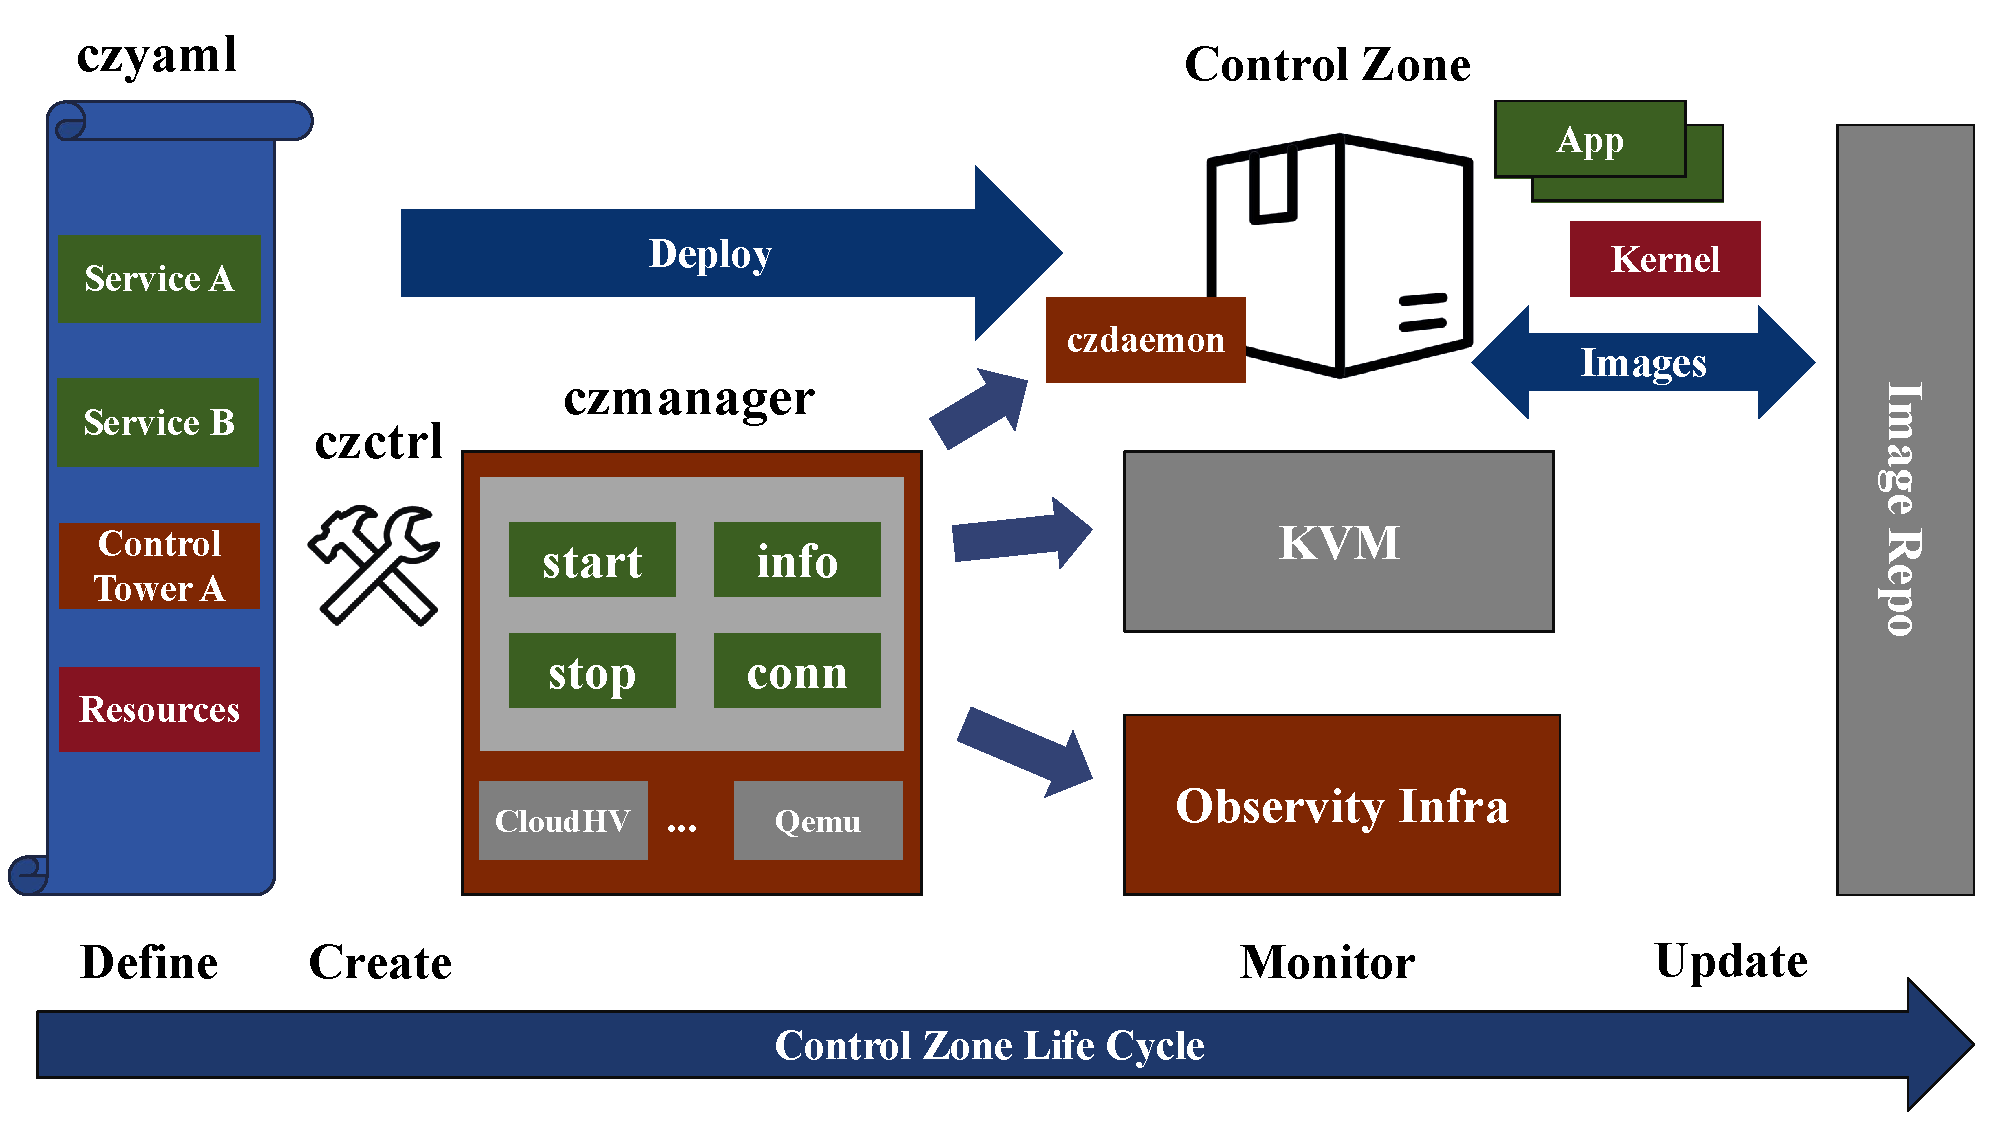
\includegraphics[width=0.9\textwidth]{cz_components}
    \bicaption{\quad Control Zone组件结构}{\quad Components of Control Zone}
    \label{fig:cz_components}
\end{figure}

1)czyaml:Control Zone定义。czyaml包含Meta、Guest、Resource三部分,其中Meta包含一些元数据,用以区分不同的Control Zone。Guest部分则用于声明运行环境,包括使用的系统、调度器及根文件系统。Resource部分用于声明隔离的资源,包括常见的CPU、Memory以及Intel RDT子系统中的LLC和内存带宽。

2)czmanager:Control Zone管理。czmanager负责Control Zone的实际管理, 包括创建、查看、启动、暂停、更新以及清除等完善的生命周期管理。过程中czmanager主要负责维护Control Zone的状态,并协同底层虚拟化运行时实现最终的虚拟机管理。而在可观测性上,czmanager利用了虚拟机各层次的信息生成监控配置,并与可观测性基础设施协作以实现Control Zone的持续监控。资源管理上,czmanager主要与虚拟化运行时、Linux Resctrl及Cgroup子系统交互,根据czyaml中的定义实现Control Zone的资源隔离。

3)czdaemon:Control Zone守护程序。czdaemon运行在每个Control Zone之中,在启动阶段主要用来信息获取与状态探测。而在启动完成之后,作为Control Zone内外沟通的桥梁,对外与czmanager交互,以接收命令,对内则直接与容器运行时交互,实现镜像及容器的管理。

4)czctrl:用户命令行工具。czctrl是所有请求的入口,能够解析用户输入的命令并验证czyaml配置,随后再与czmanager交互以达成用户管理Control Zone和任务的目的。

5)镜像存储服务:容器及其他静态资源管理。应用与BPF Scheduler都以OCI容器镜像的形式保存在镜像存储服务中,并通过容器的形式运行,同时为方便其他静态资源的管理,预编译内核及根文件系统也保存在精简容器镜像的中交给镜像存储服务管理。

\section{Control Zone设计}

% Control Zone Yaml
% Control Zone关键流程的执行过程
% - start
% - stop
% - update
% - remove
% Control Zone容器的管理流程
% - add
% - delete
% Control Zone调度的流程
% - czctrl的资源限制
% - chsd的策略控制
% - sched ext的策略控制

Control Zone Yaml提供了丰富的资源隔离配置~\ref{tab:cz_config},隔离性围绕三个层次进行设计,首先,虚拟机本质上是一种特殊的进程,Linux中提供了Cgroup技术来隔离进程的资源,因此在配置文件中,允许声明Cgroup配置参数,来限制如虚拟机能够使用的CPU核心等,同时作为进程,也能够被Linux Resctrl子系统管理,从而构造LLC与内存带宽的隔离。其次,虚拟机本身还由Hypervisor管理,而大部分Hypervisor都提供了额外的资源隔离机制,主要体现在硬件模拟上,如对于CPU,可以限制提供给虚拟机使用的CPU feature,而对于其他设备,则提供了对virtio net设备的收发速度及virtio blk设备的读写速度的控制。最后,虚拟机内的guest os本身也能够提供一些隔离机制,在Control Zone中能够通过调度子系统来对不同的任务进行隔离,如将任务划分到不同优先级的调度队列中, 从而在相同调度队列上构造任务粒度的隔离性,这一配置通常与混部任务一同设置。

\begin{table}
    \bicaption{\quad Control Zone配置列表}{\quad Control Zone Config}% caption
    \label{tab:cz_config}
    \footnotesize% fontsize
    \setlength{\tabcolsep}{4pt}% column separation
    \renewcommand{\arraystretch}{1.5}% row space 
    \centering
    \begin{tabular}{lcc}
        \hline
        %\multicolumn{num_of_cols_to_merge}{alignment}{contents} \\
        %\cline{i-j}% partial hline from column i to column j
        类型 & 配置 & 说明\\
        \hline
        Meta & name & Control Zone名称 \\
        & workdir & Control Zone工作目录,存放日志及其他配置 \\
        & share\_folder(可选) & 额外共享给Control Zone的目录 \\
        & label & 标签,数个key-value对 \\
        & vrun & 虚拟机运行时,可选CloudHypervisor、Qemu或Libvirtd \\
        Guest & kernel(可选) & Control Zone使用的内核,从镜像存储拉取 \\
        & initramfs(可选) & 初始化内存文件系统,默认情况下不使用 \\
        & rootfs(可选) & Control Zone使用的根文件系统,从镜像存储拉取\\
        & kcmdline(可选) & 内核的运行命令 \\
        Resource & [cgroup] & 虚拟机Cgroup配置 \\
        & cpu.max & 最大CPU使用限制 \\
        & cpu.max.burst & 最大突发CPU使用限制 \\
        & cpuset.cpus & CPU亲和性 \\
        & cpuset.mems & 内存节点亲和性 \\
        & [hypervisor] & 虚拟机hypervisor配置 \\
        & cpu features& vCPU可用的特性\\
        & bw\_size & 设备带宽大小(byte/s)\\
        & bw\_one\_time\_burst & 设备突发带宽大小(byte/s)\\
        & bw\_refill\_time & 设备带宽恢复时间(ms)\\
        & ops\_size & 设备操作速度(op/s)\\
        & ops\_one\_time\_burst & 设备突发操作速度(op/s)\\
        & ops\_refill\_time & 设备操作速度恢复时间(ms)\\
        \hline
    \end{tabular}
\end{table}

运行时可定制调度的沙箱提供了create、start、stop、remove、update四种操作来管理Control Zone的生命周期,在不同操作下Control Zone的状态变化如图~\ref{fig:cz_state}所示,其中 sync 过程由czdaemon完成,而对于不能直接达到的状态,czmanager会试图进行多次状态切花以达到目标状态,而对于不可达的状态,czmanager将会提示操作非法。update操作对于状态的影响取决于所更新的参数,如对内核的修改将要求Control Zone进行重新启动。

\begin{figure}[!htbp]
    \centering
    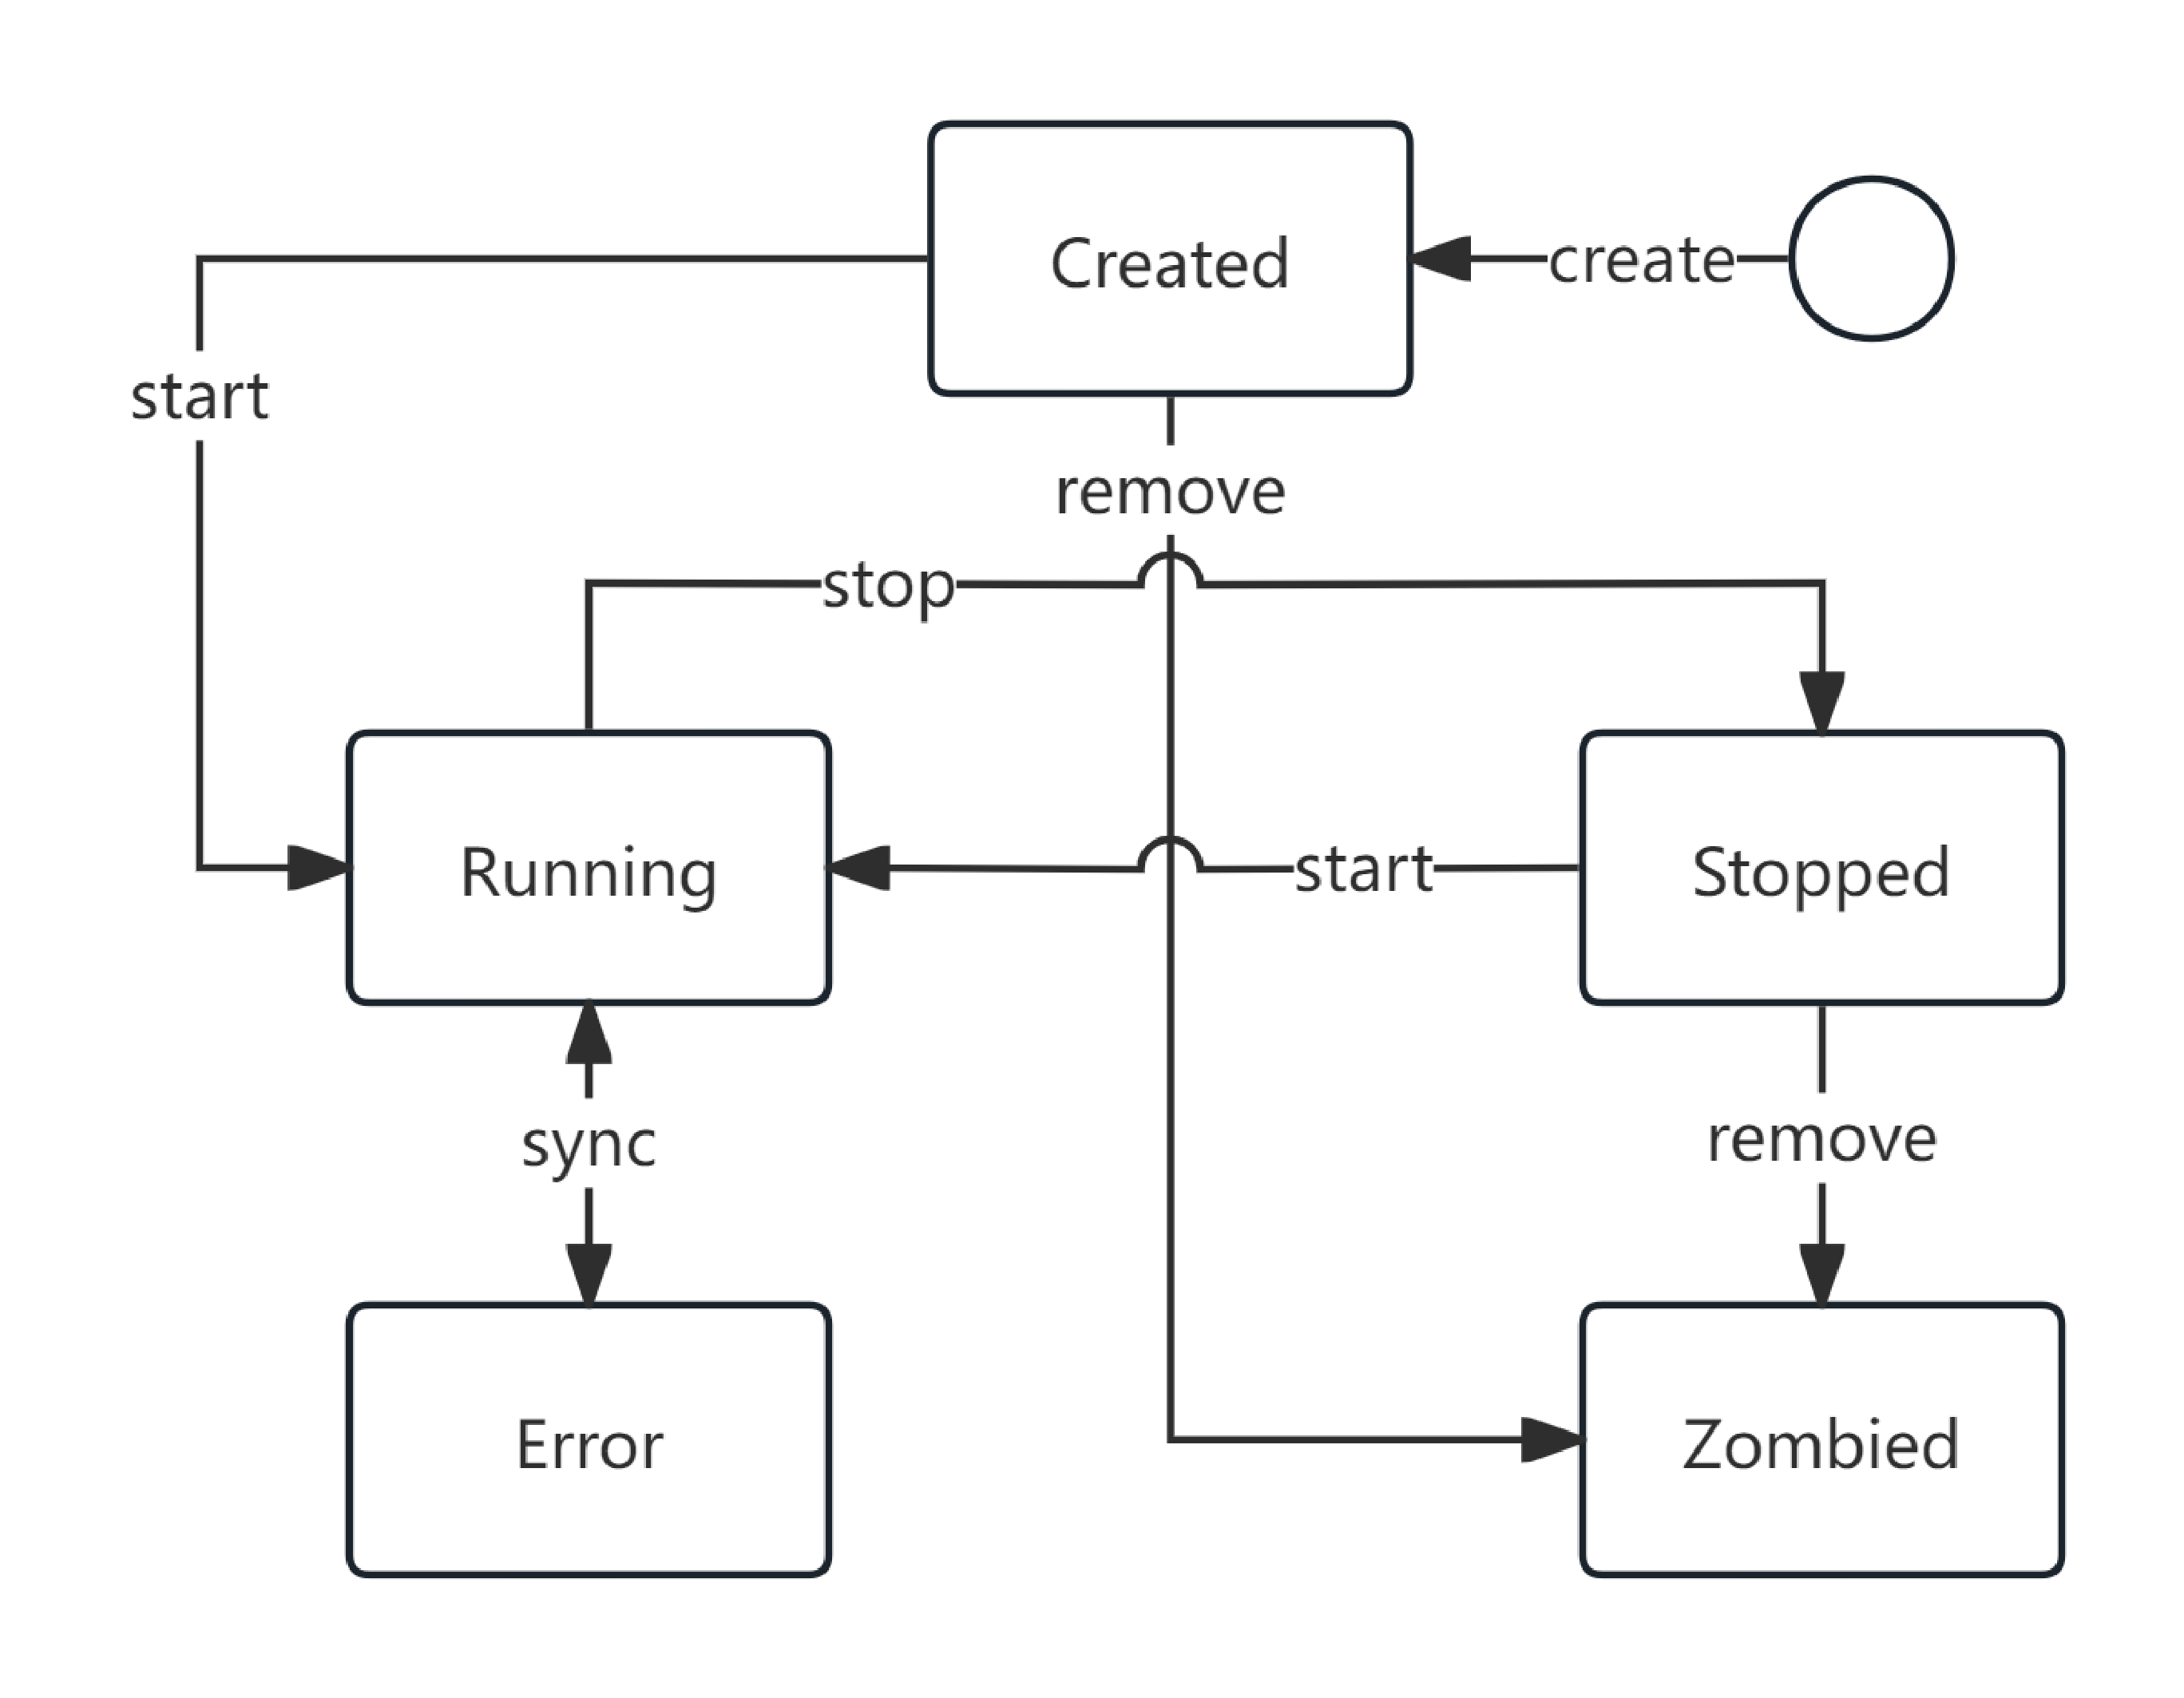
\includegraphics[width=0.6\textwidth]{cz_state}
    \bicaption{\quad Control Zone状态迁移}{\quad State of Control Zone}
    \label{fig:cz_state}
\end{figure}

Control Zone的创建流程如图~\ref{fig:cz_create}所示,过程中首先进行配置的合法性监测,创建过程中的检测主要判断资源是否重复分配,如对于cpuset,czmanager会检查全局的cpu mask来判断cpuset的设置是否合法。随后进行工作目录的创建,用来单独保存每个Control Zone的关键数据,如根文件系统等。创建过程仅为虚拟机的启动做好准备,而并不会启动虚拟机,相当于为虚拟机的启动预留了空间。

\begin{figure}[!htbp]
    \centering
    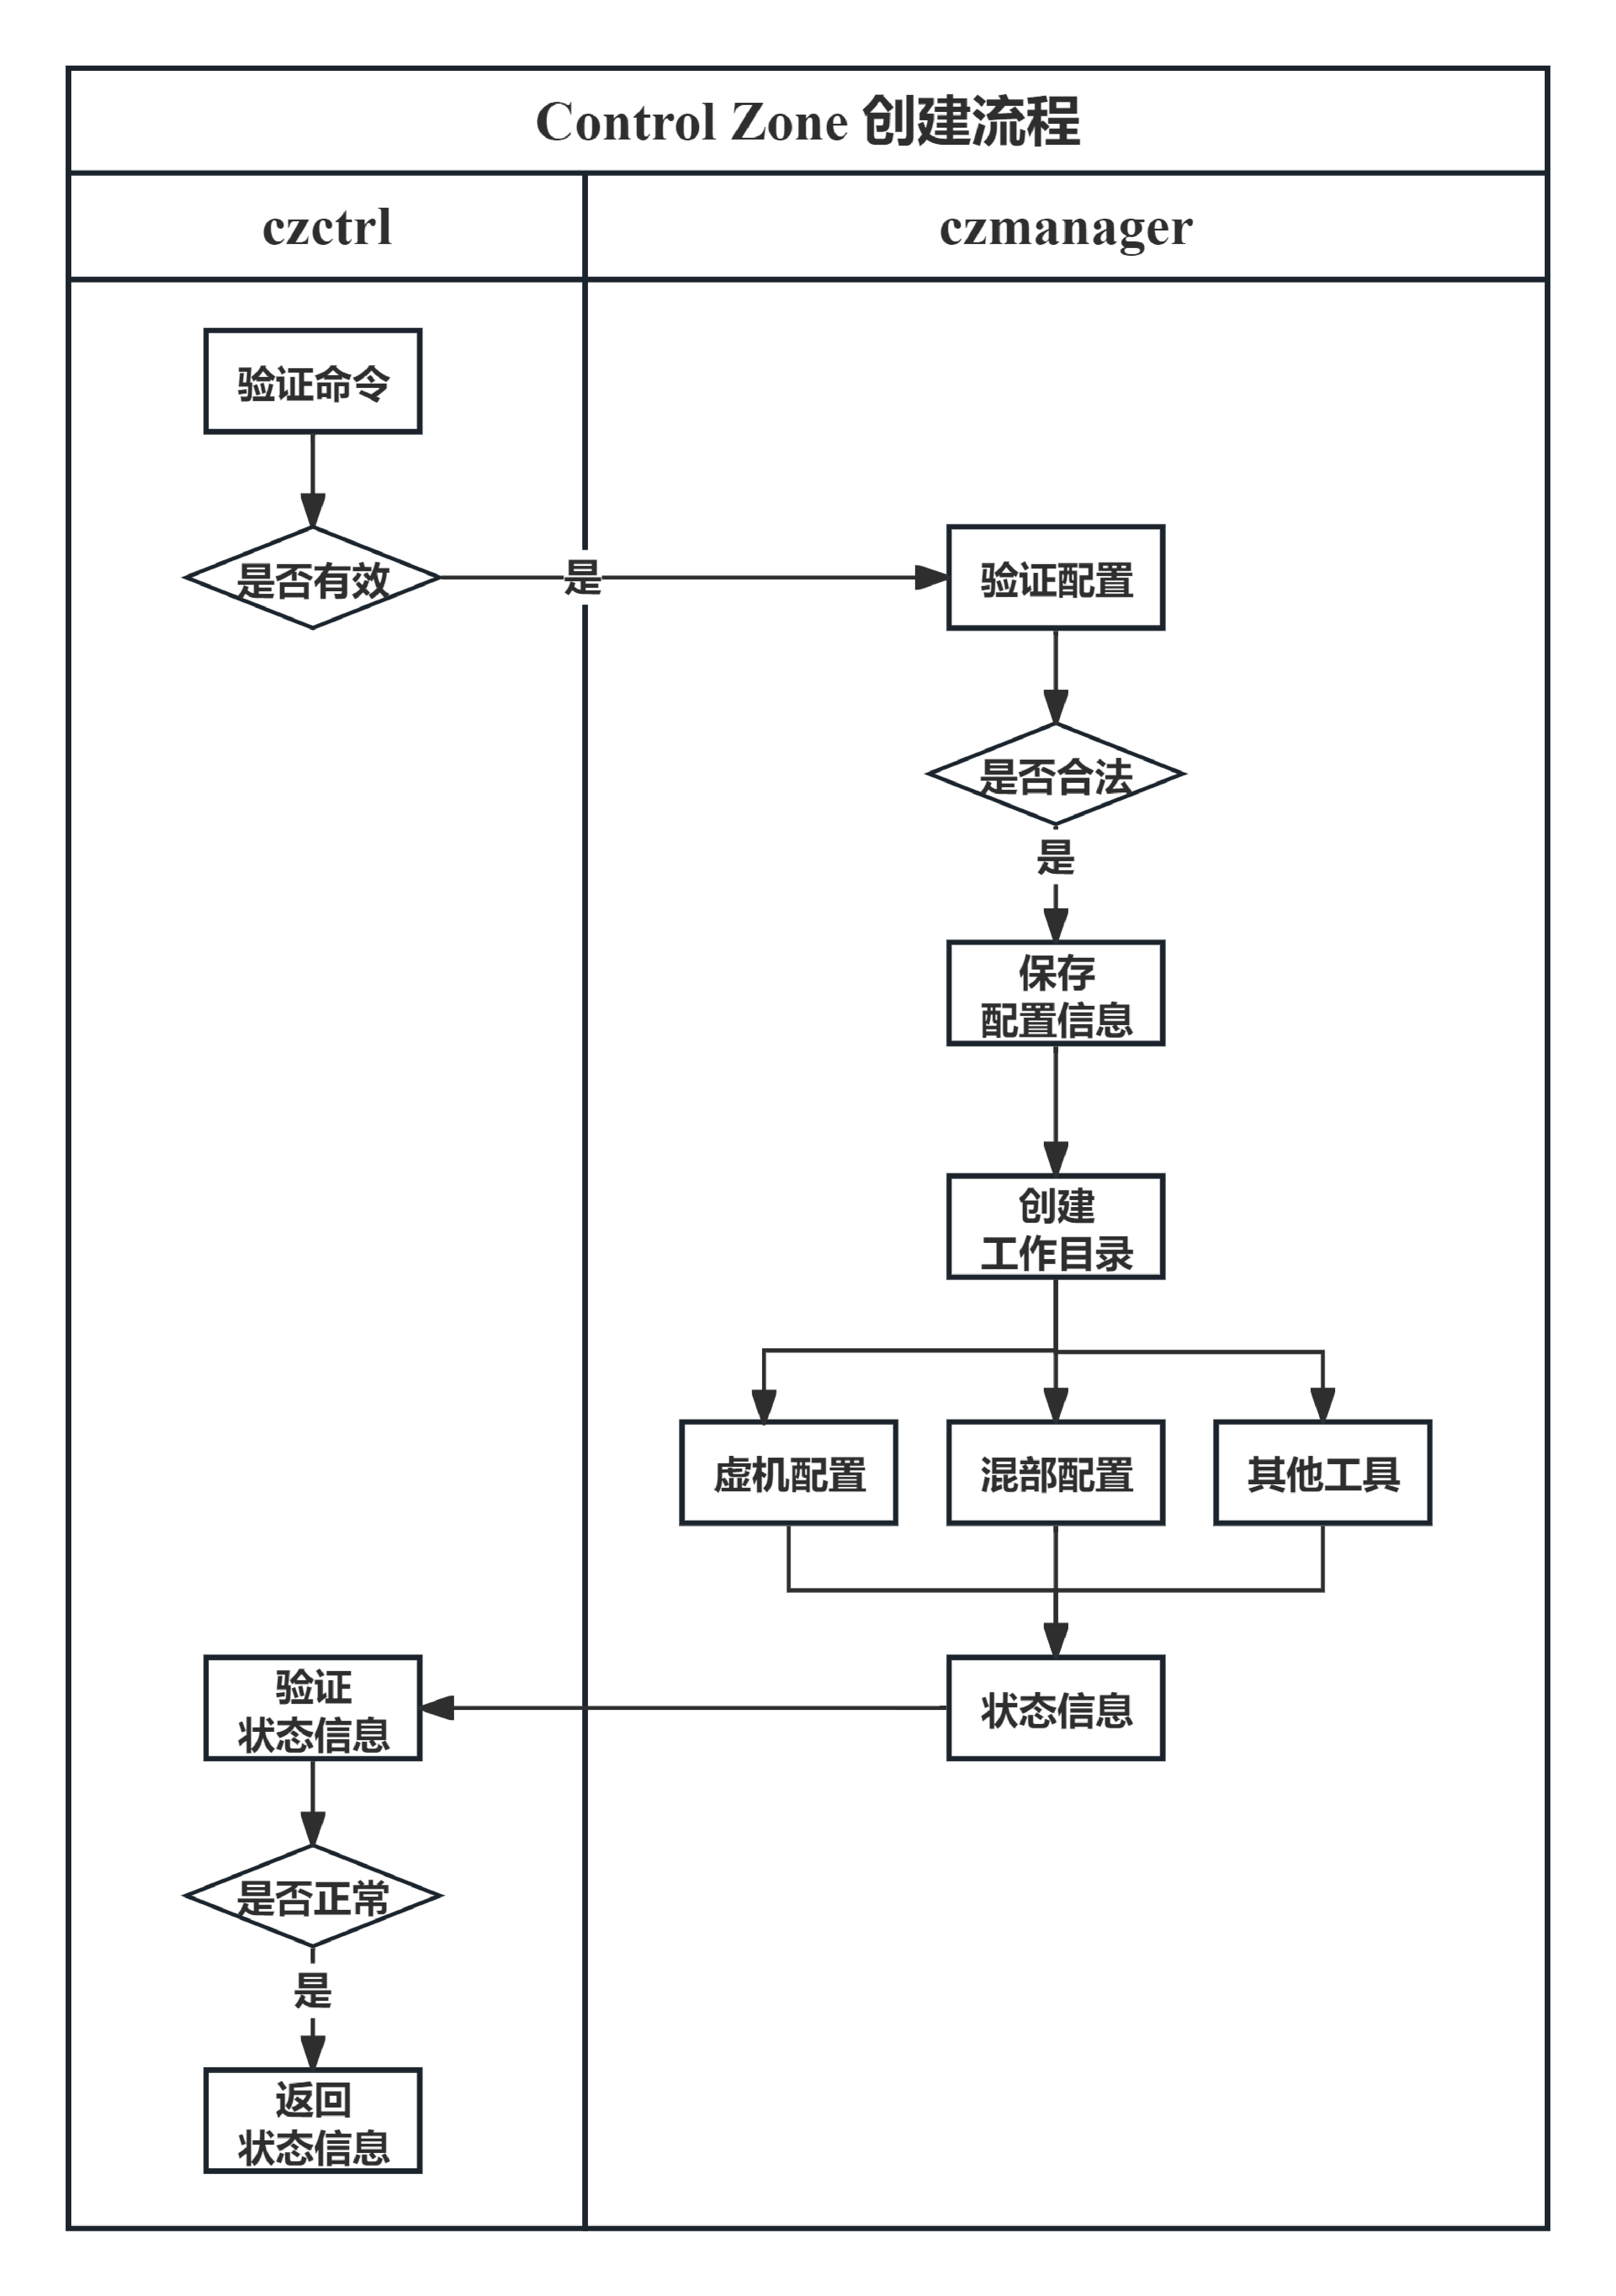
\includegraphics[width=0.5\textwidth]{cz_create}
    \bicaption{\quad Control Zone创建流程}{\quad Create Control Zone}
    \label{fig:cz_create}
\end{figure}

Control Zone的启动流程如图~\ref{fig:cz_start}所示,过程中首先进行配置的合法性监测,如判断状态迁移是否合法、验证资源是否重复分配,对于一个已经创建的Control Zone,其预留的资源并不是严格进行保护的,因此在启动时其资源可能已经被占用,此时需要涉及重新更新Control Zone的资源配置。而在一切准备就绪以后,czmanager会按照配置要求,调用目标虚拟化运行时来启动虚拟机,而在虚拟机启动完毕之后,czdaemon会检测是否有已经提交的任务,并依次在后台进行执行,随后通知czmanager虚拟机状态的变化,czmanager在收到信号之后,Control Zone的启动过程就完成,而随后czmanager会根据配置来选择为Control Zone同步观测配置。

\begin{figure}[!htbp]
        \centering
        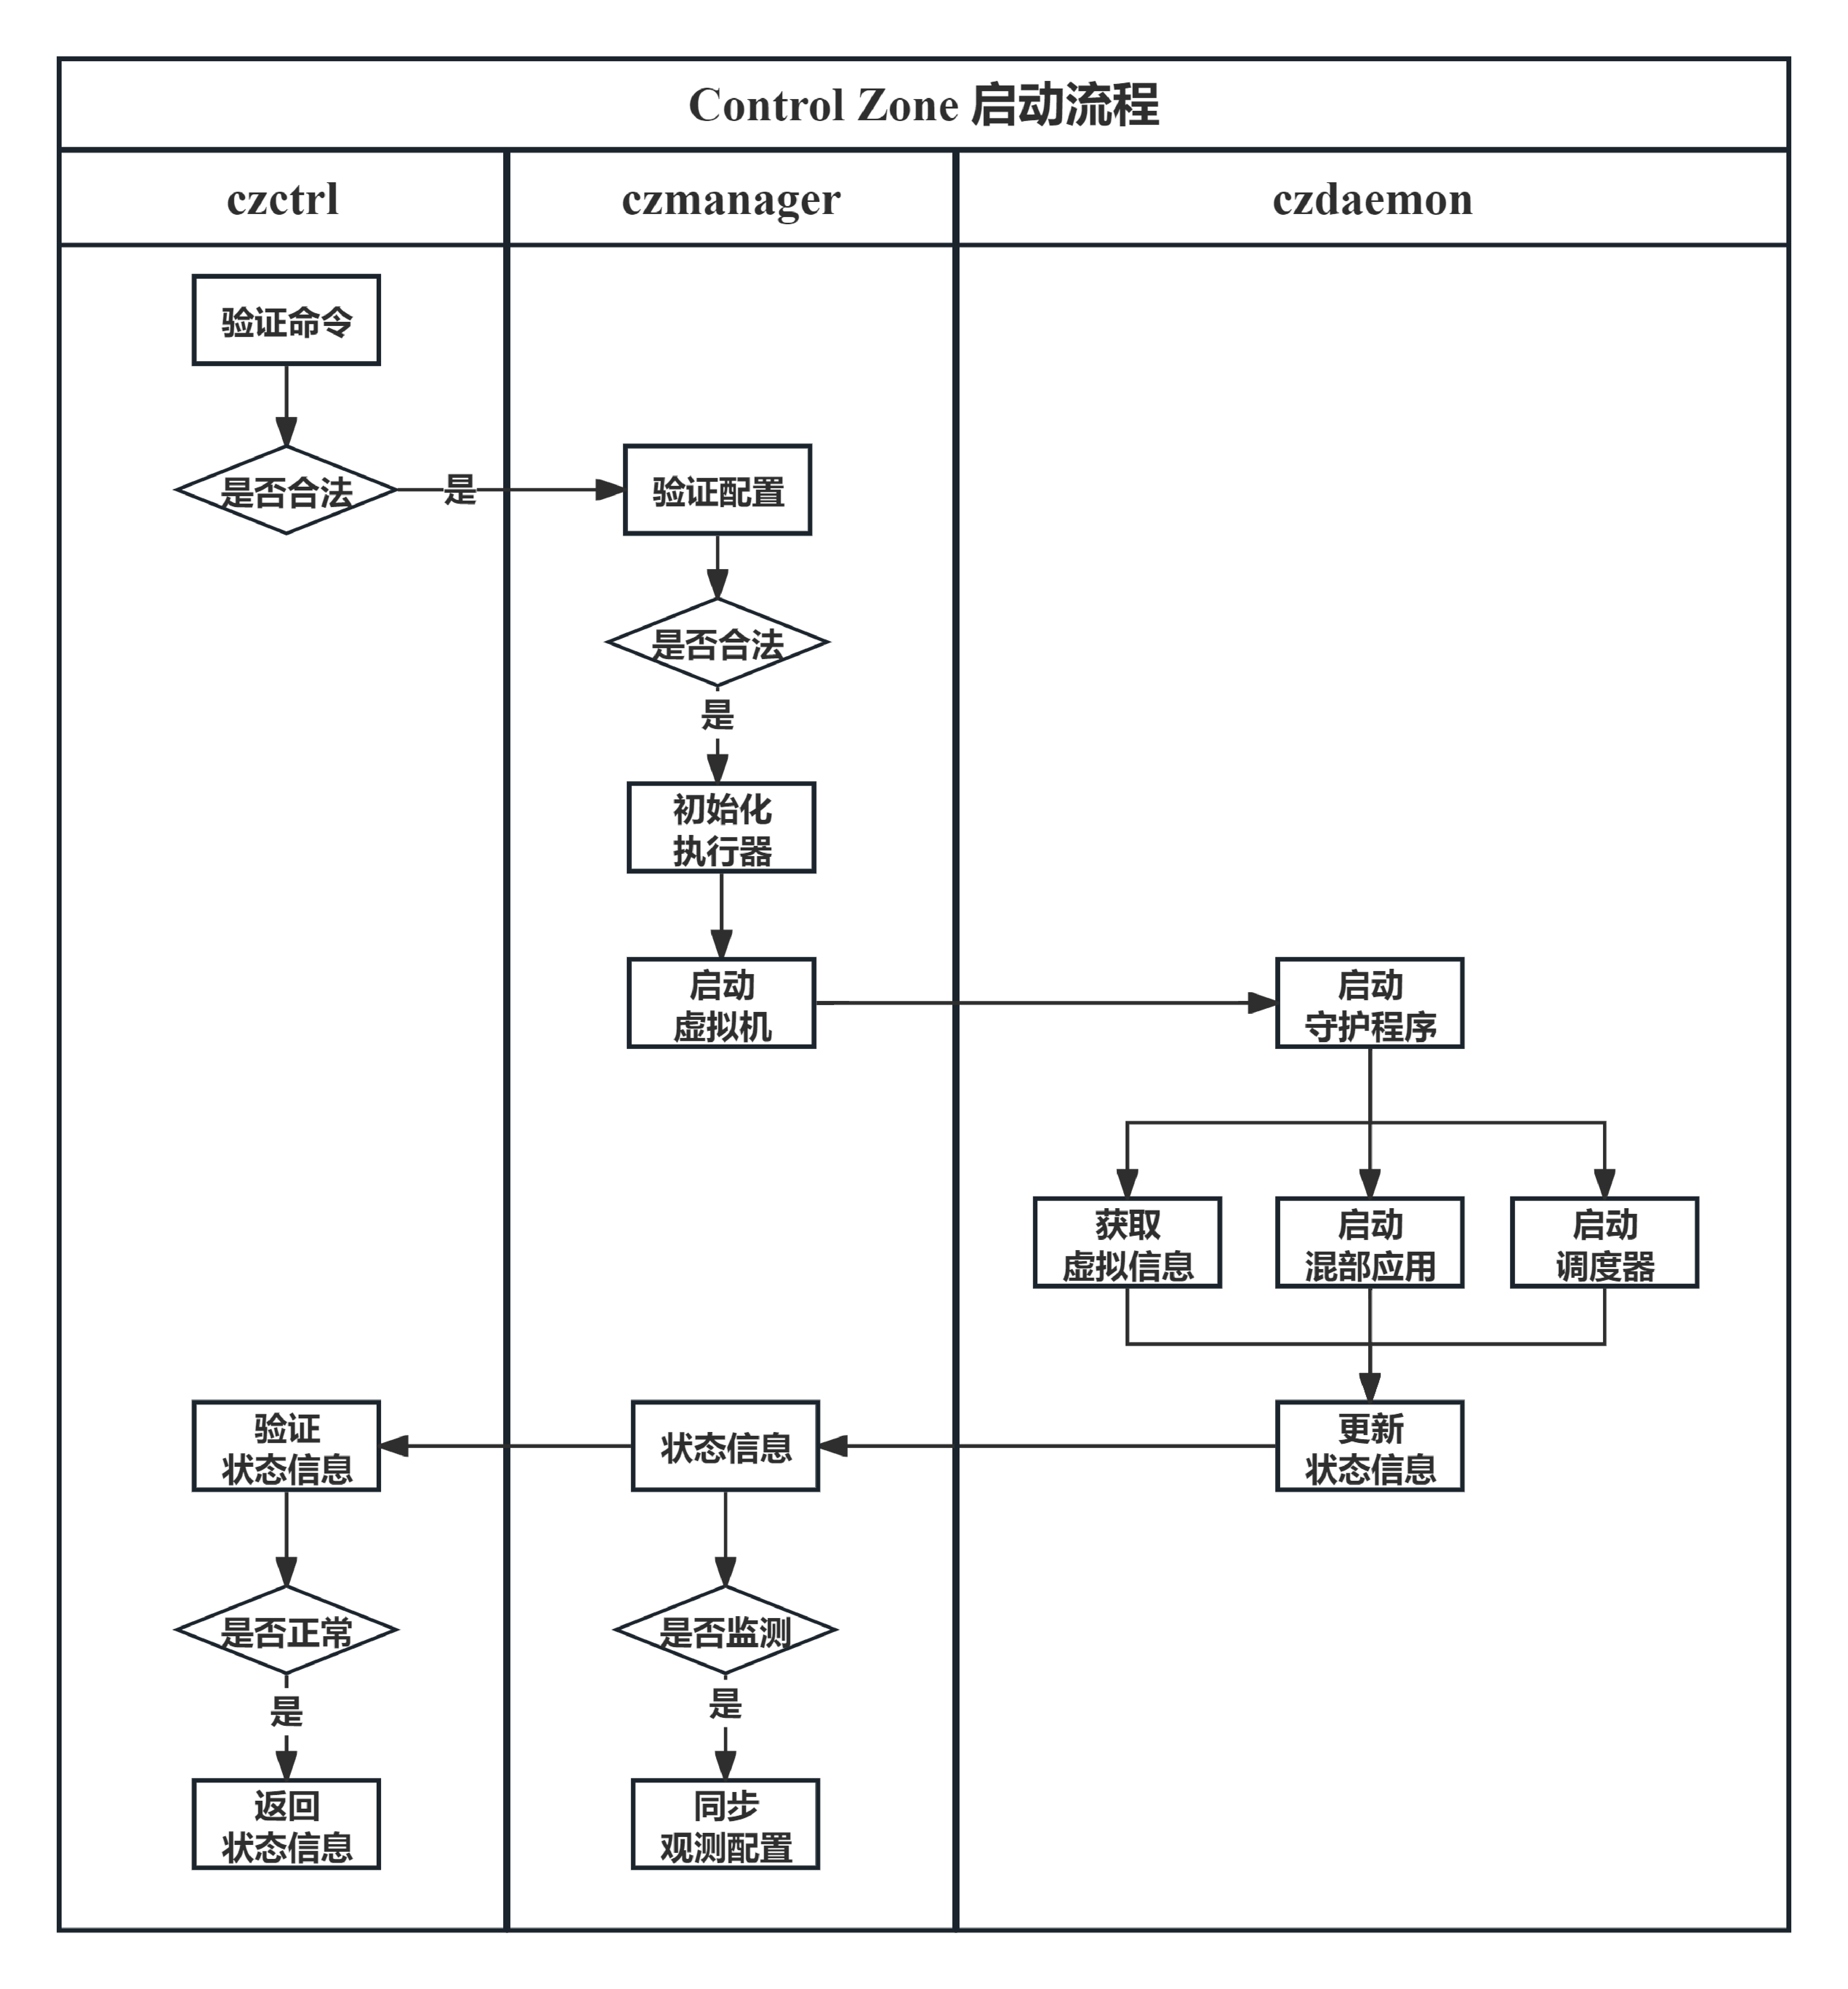
\includegraphics[width=0.6\linewidth]{cz_start}
        \bicaption{\quad Control Zone启动流程}{\quad Start Control Zone}
        \label{fig:cz_start}
\end{figure}

Control Zone的停止过程如图~\ref{fig:cz_stop}所示,考虑停止之后存在重新启动的可能,因此沙箱采用了较为保守的关闭策略。关闭过程中需要czmanager与czdaemon协同合作,在验证配置之后,czmanager首先会通知czdaemon进行关闭处理,而czdaemon在接收到关闭信号之后,会对当前系统的状态进行保存,如必要的信息、混部应用状态等,再将托管的任务关闭,随后再通知czmanager, 直到此时czmanager才会真正地调用执行器来关闭虚拟机,并在必要时通知可观测性基础设置停止监测。Control Zone停止之后仍然会保有相关的资源记录,便于后续重新启动。

\begin{figure}[!htbp]
    \centering
    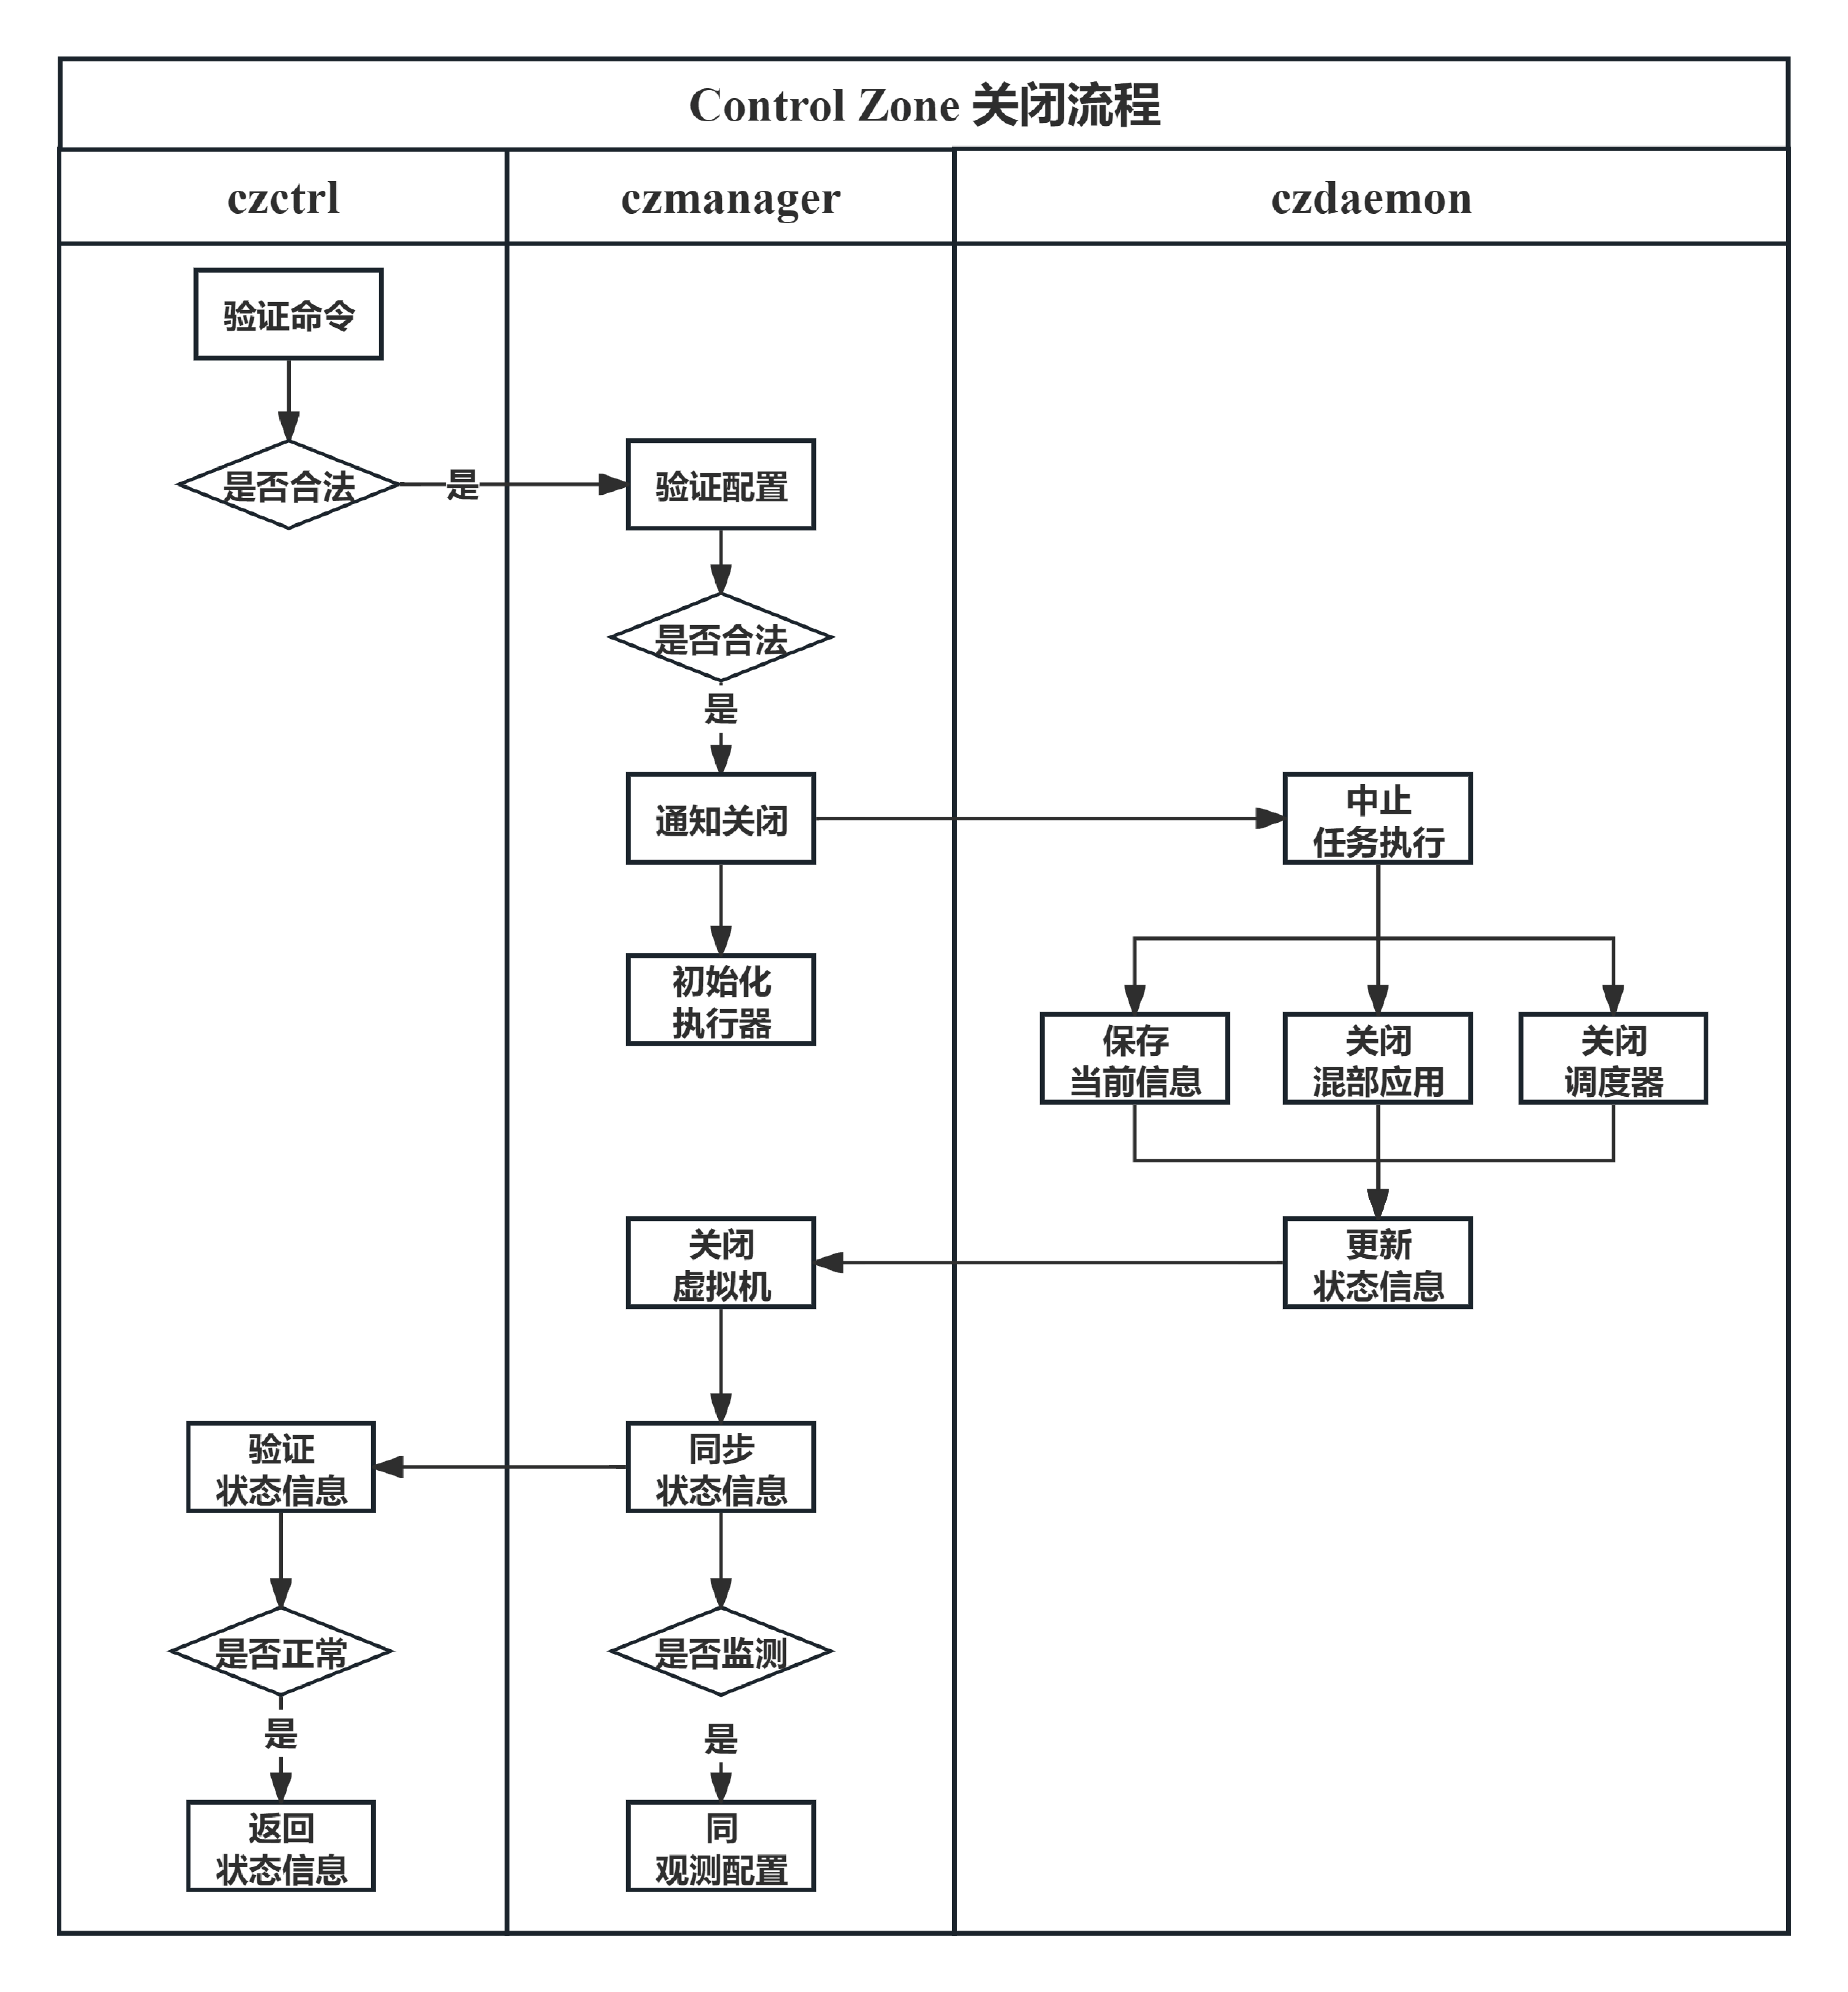
\includegraphics[width=0.6\textwidth]{cz_stop}
    \bicaption{\quad Control Zone关闭流程}{\quad Stop Control Zone}
    \label{fig:cz_stop}
\end{figure}

Control Zone的更新过程如图~\ref{fig:cz_update}所示,Control Zone Yaml中的绝大部分字段都允许被更新,一些字段的更新由czmanager调用资源管理接口完成,如修改cgroup或resctrl等字段中的内容,czmanager发现只有这些字段被修改时,就会重新修改资源隔离配置,并调用各个资源管理接口来进行实施。 而部分字段则会涉及到Control Zone的重新启动,如对Guest中的内核、根文件系统等字段进行修改,czmanager检测到这些字段发生修改后,就会进如重新启动的流程,并在关闭虚拟机之后,实施相关更新内容,再启动虚拟机。更新完毕后,观测配置可能会过时,因此必要时czmanager还会与可观测性基础设施同步观测配置的变化。

\begin{figure}[!htbp]
    \centering
    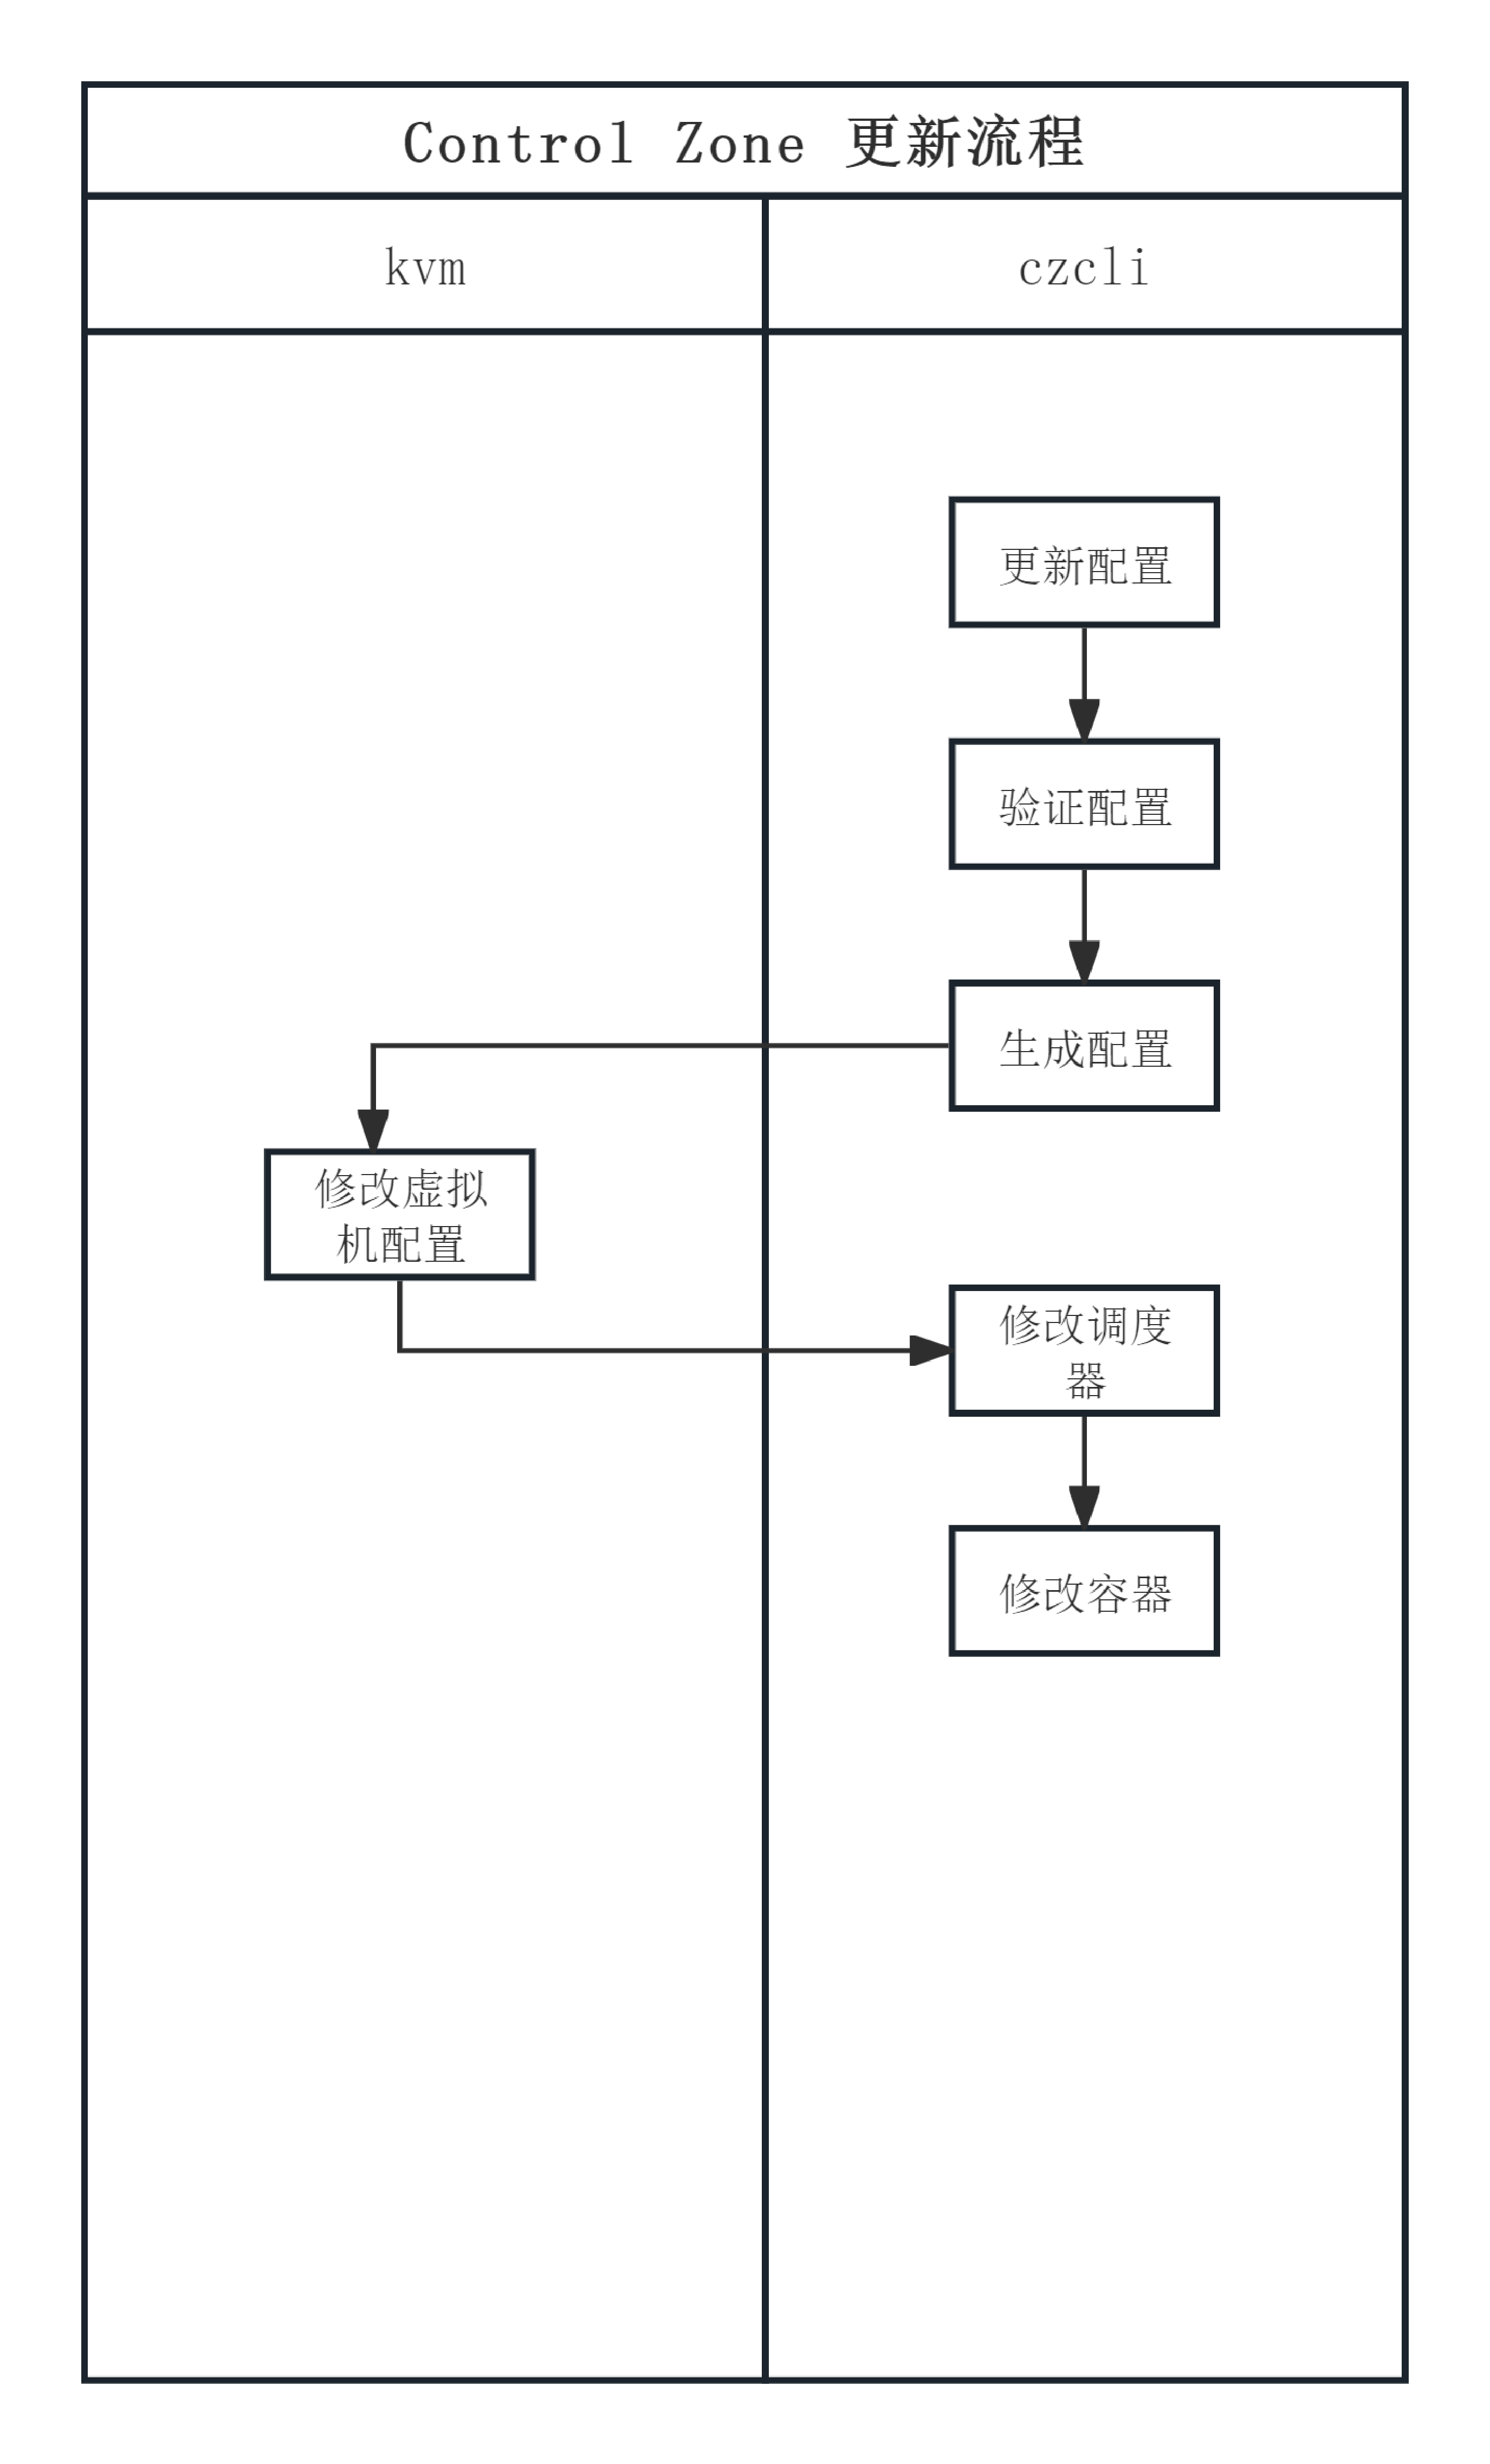
\includegraphics[width=0.7\textwidth]{cz_update}
    \bicaption{\quad Control Zone更新流程}{\quad Stop Control Zone}
    \label{fig:cz_update}
\end{figure}

Control Zone的删除过程如图~\ref{fig:cz_remove}所示,通常只有已经停止的Control Zone能够被删除,而为简化操作,当Control Zone为其他状态时,此时进行删除操作时会首先将Control Zone的状态转化为停止状态,在进行删除操作。Control Zone的除了工作目录的销毁外,还会回收已经分配的资源。

\begin{figure}[!htbp]
    \centering
    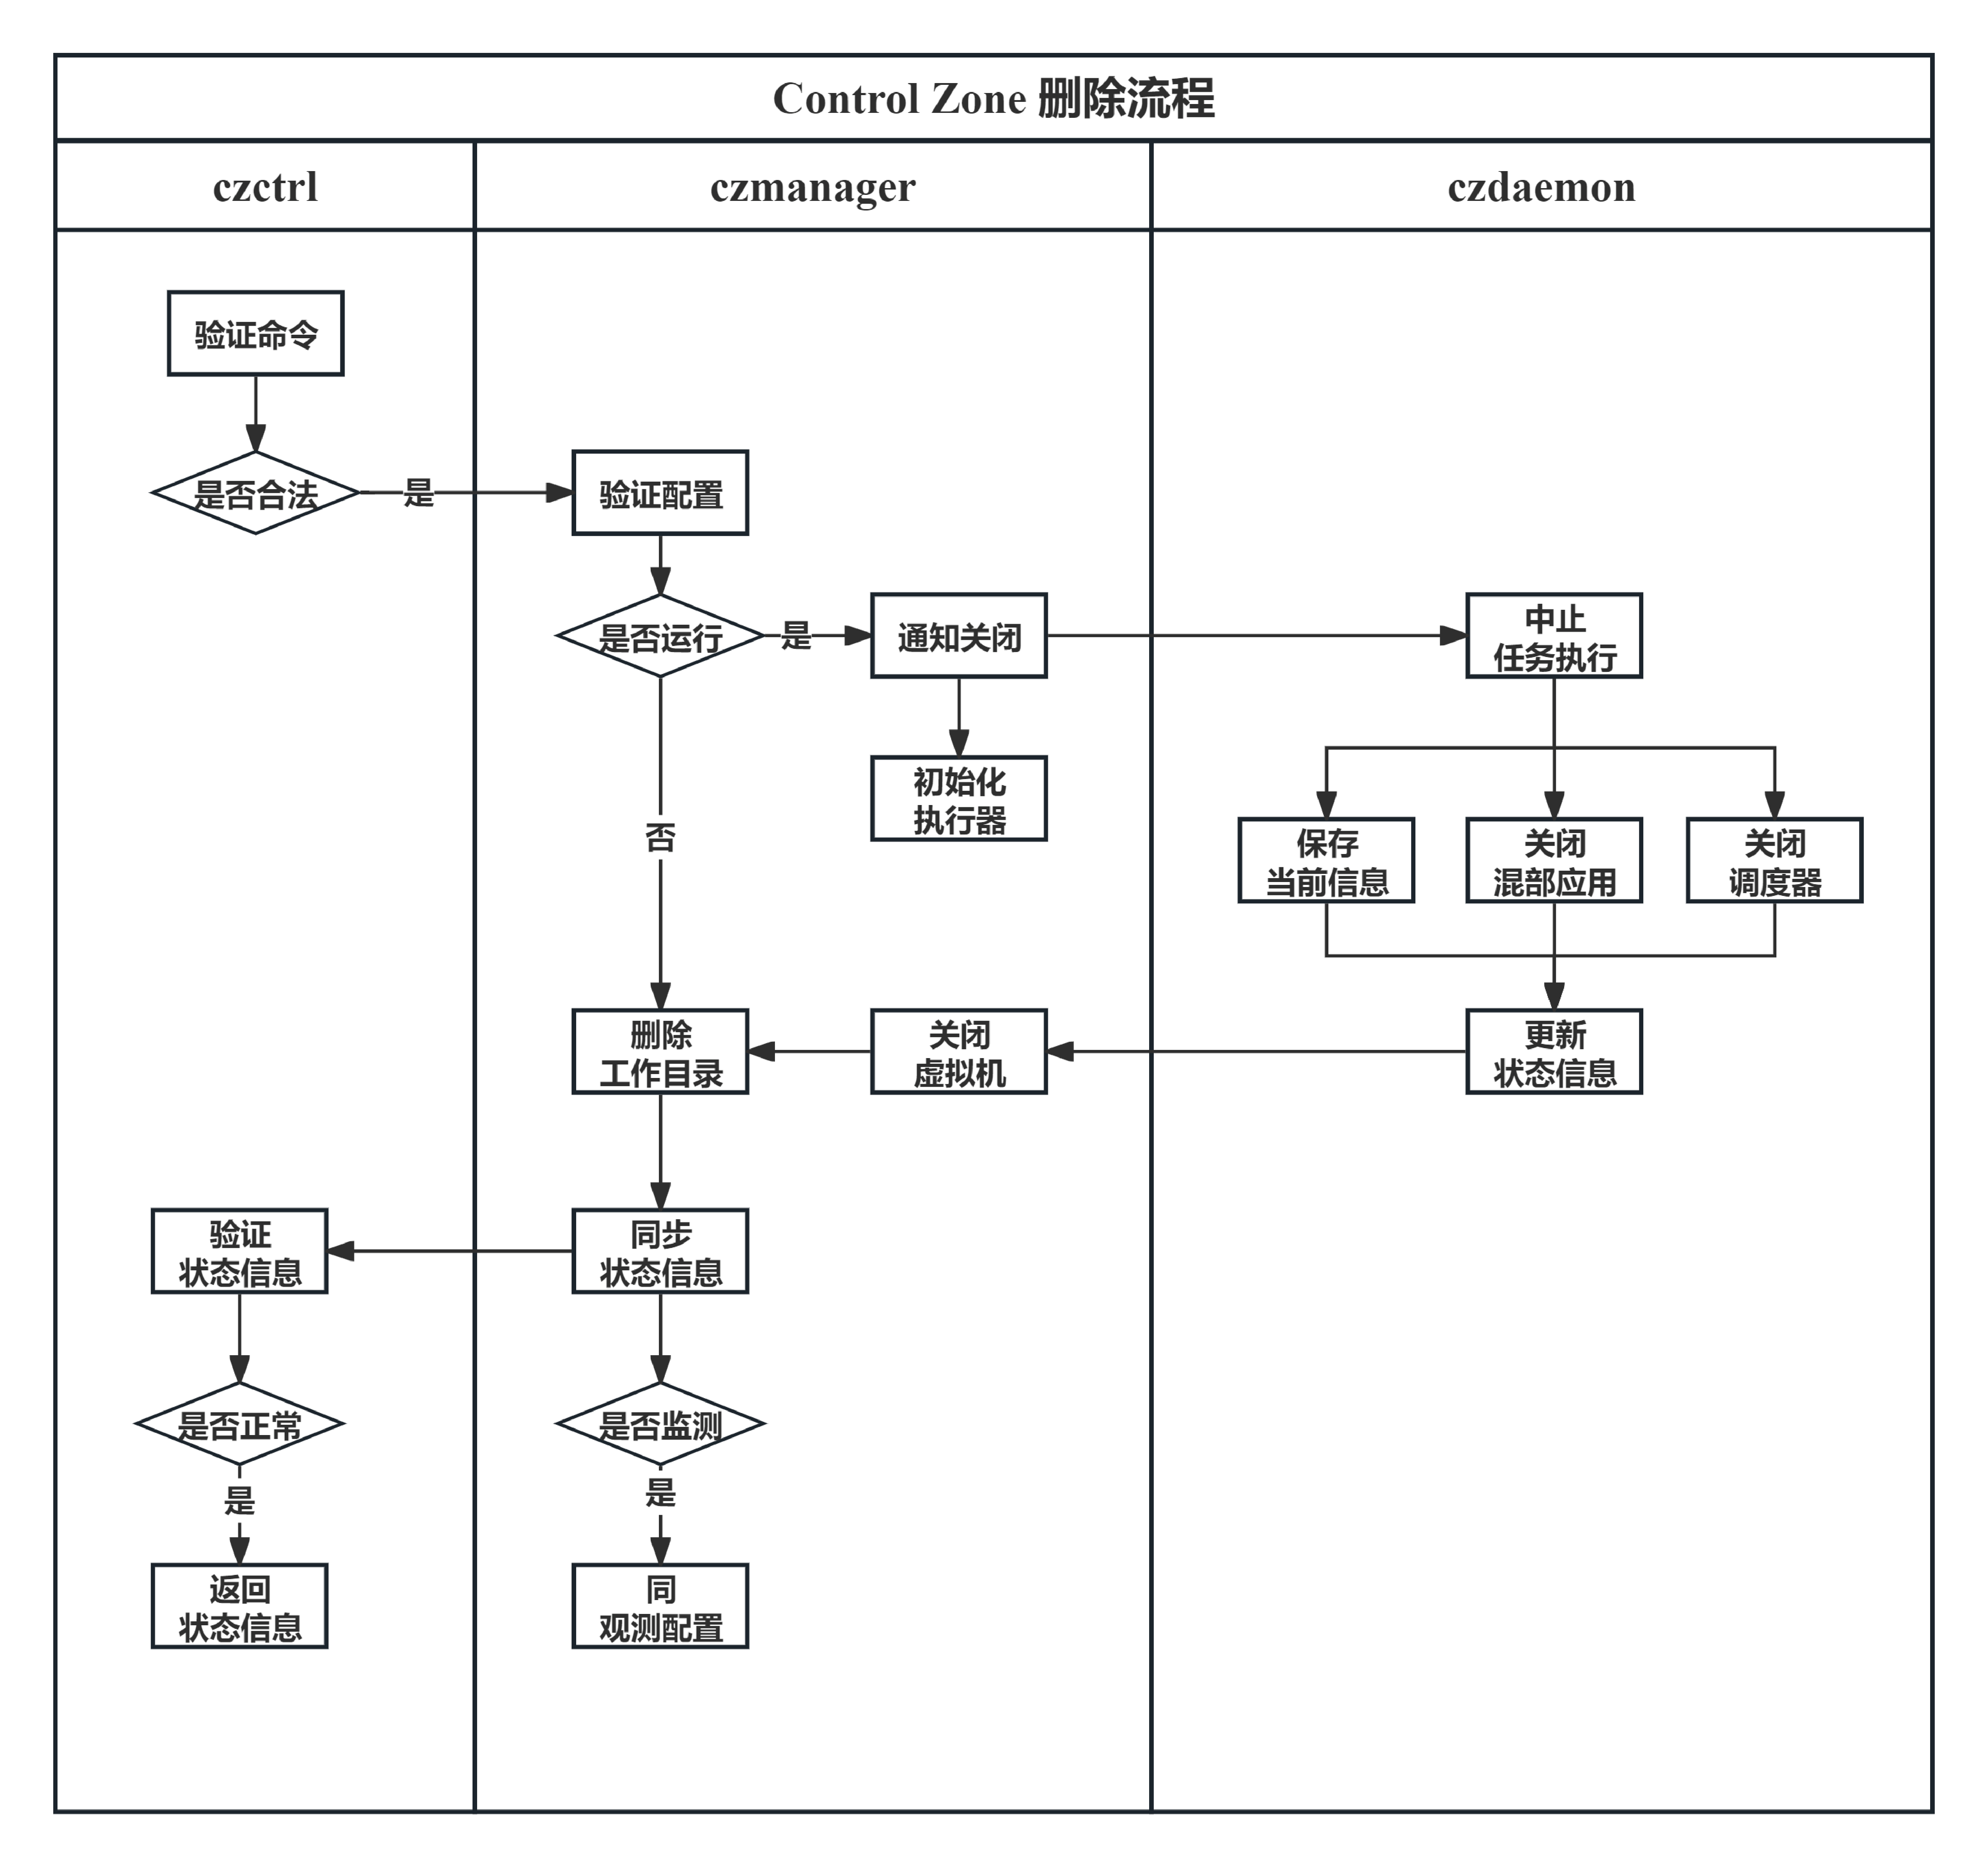
\includegraphics[width=0.7\textwidth]{cz_remove}
    \bicaption{\quad Control Zone删除流程}{\quad Remove Control Zone}
    \label{fig:cz_remove}
\end{figure}

\section{Control Zone实现}

% 隔离性实现
% 内核裁切
% hypervisor选择
% 系统功能要求
% 镜像共享

% 1)czyaml: 定义一个Control Zone。完整的czyaml包含三个部分,第一个部分是Meta,其与Control Zone的管理密切相关,核心是Control Zone的ID、Name、Label、以及vRun,其中ID与Name用以区分不同的Control Zone,而标签由用户自定义,用来描述Control Zone的属性,最后VRun用来指定Control Zone所使用的虚拟化环境,默认使用轻量级虚拟化环境CloudHypervisor。第二个部分是GuestEnv,用来声明Control Zone所使用的运行环境,包括内核、BPF调度器、根文件系统、以及可选的initramfs,内核可以来自于镜像存储服务,也可以选择基于基准配置自行编译的本地内核,BPF调度器则来自于镜像存储服务,需要对其初始化参数进行相关的配置。第三个部分是Resource,用来声明Control Zone要占用的资源,除常规的虚拟机资源如CPU、Memory、BLK IO、Net IO之外,还包括了Resctrl子系统中的末级缓存路数以及内存带宽。

\subsection{虚拟化开销优化}

Control Zone引入虚拟化出于两个原因。首先,Control Zone需要一个较强的隔离环境,引入虚拟化一方面增强了隔离效果,同时也能够基于Hypervisor来提供更多的资源限制手段。其次,Control Zone中基于调度子系统来协调多任务的执行,使用虚拟机一方面能够提供场景上的限制,如有限的硬件资源,有限的竞争应用等,其次,修改任务的调度信息是较为风险的行为,如过设置不当有可能引发整个系统的性能劣化,而利用虚拟机能够防止这种风险的扩散。

而为减少引入虚拟化所产生的开销,沙箱实现时从两个方面入手。一方面,围绕虚拟机系统环境进行裁切,首先,对于内核,Control Zone内核中只保留了必要的virtio驱动,以及运行容器、BPF子系统与Sched Ext调度类的最小支持,其次,对于启动过程,由于Control Zone内核环境足够简单且不用考虑灵活性,因此在启动过程中跳过initramfs阶段,并直接挂载根文件系统,最后,对于根文件系统,Control Zone根文件系统基于轻量Linux发行版Aline\citep{alpine}构建,使用busybox作为基础工具,并同时使用轻量级C标准库的musl,而在容器运行时上,选择基于C语言的crun\citep{crun}作为容器运行时,相较于使用Go语言开发的runc,crun在启动容器上的开销降低了49.4\percent,同时占用的内存也更少。另一方面,在虚拟化运行时上,沙箱默认使用更轻量化的虚拟化运行时CloudHypervisor,CloudHypervisor使用Rust语言开发,相较于Qemu,主要优化了设备虚拟化的部分,去除了大量与云场景无关设备模拟,提示了Hypervisor的初始化速度,并减少了运行时的额外内存开销。如图~\ref{fig:boot_time}所示,经过如上优化之后,相较于使用Qemu启动的Alpine默认内核,使用Cloud Hypervisor启动的Control Zone内核在启动开销上降低了86\percent,裁切力度更激进的Firecracker内核相较于Control Zone进一步降低36\percent的启动开销,对比内核启动日志,这部分开销主要来自于Control Zone中支持容器及BPF子系统的额外功能,这些功能对于本设计而言是必须的,实际上在实验环境中,这部分时间约为0.15秒。不同于Firecracker,Control Zone在设计中并不与应用完全耦合,即便任务退出,Control Zone仍然会保留一段时间,在任务数量足够多时,Control Zone并不会频繁地启动,因此这部分开销是可以接受的。

\begin{figure}[!htbp]
    \centering
    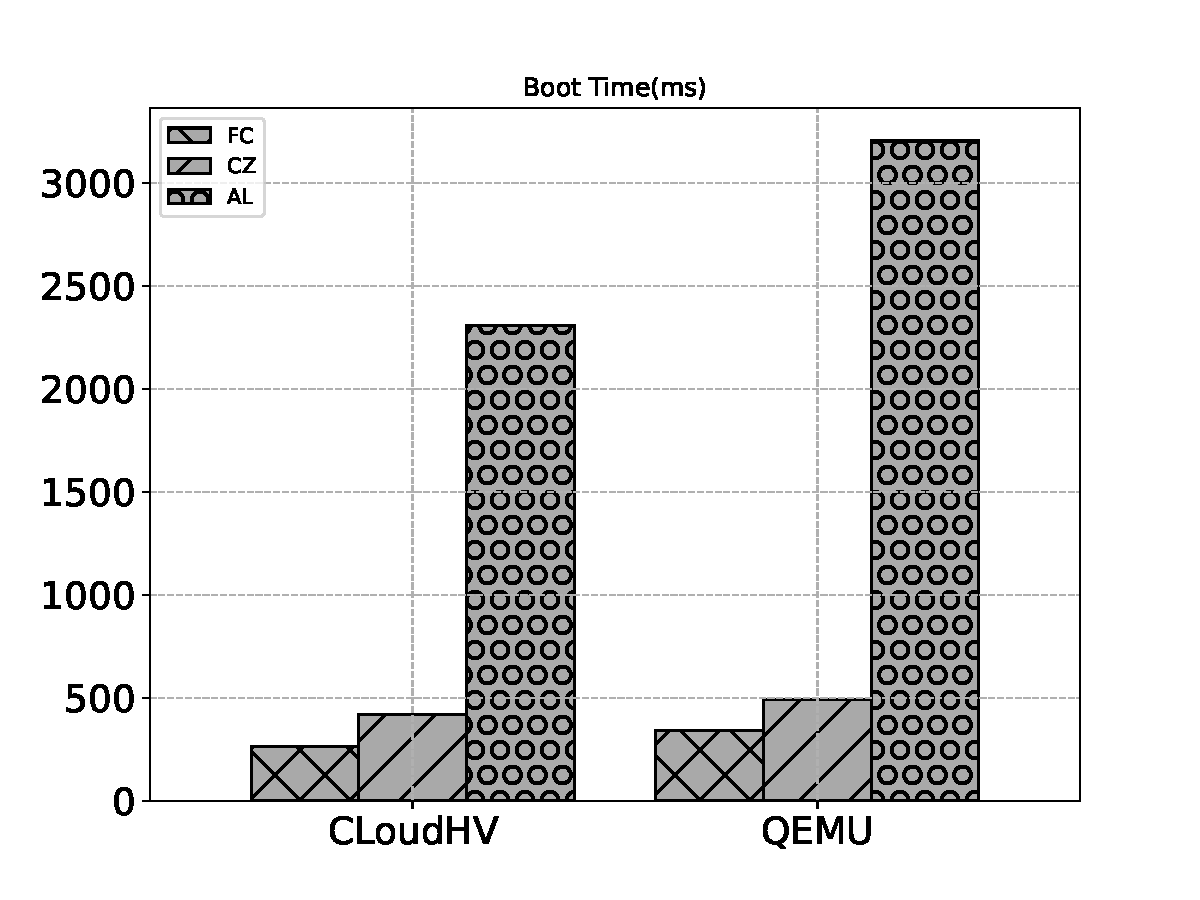
\includegraphics[width=0.7\textwidth]{boot_time}
    \bicaption{\quad 启动时间为引导至运行init程序的时间,比较Firecracker(FC)、Control Zone(CZ)、Alpine(AL)内核,使用Cloud Hypervisor与Qemu}{\quad Boot time is the time it takes to boot to the init program. Compare Firecracker(FC), Control Zone(CZ), and Alpine(AL) kernels using Cloud Hypervisor and Qemu.}
    \label{fig:boot_time}
\end{figure}

同时为满足多样的使用需求,沙箱也兼容了Libvirt的使用。Libvirt并不是一个虚拟化运行时,而是针对多种虚拟化技术的抽象层,提供了更标准的API来对虚拟机进行管理。通过兼容Libvirt,Control Zone能够获取更多的特性,尤其在可观测性上,借助Libvirt提供的监测接口,可观测性基础设施能够以虚拟机为粒度采集多种指标信息。

\section{本章小结}

本章首先介绍了运行时调度可变的沙箱Control Zone的基本概念,以及其对数据中心中单节点混部场景的处理方式,即结合外侧虚拟机资源隔离与内部BPF Scheduler任务调度。

随后介绍了沙箱中的czctrl、czmanager、czdaemon等组件及其主要功能,并详细阐述了Contorl Zone的隔离能力以及Control Zone生命周期管理中各个组件的协作流程。

由于Control Zone中的BPF Scheduler也以容器的形式运行,因此能够和普通任务一样进行管理。因此在任务部署上,Control Zone允许将混部任务与调度策略共同部署,通过定制化调度来解决混部下的性能劣化问题。

最后则介绍了Control Zone在实现中为解决引入虚拟化带来的开销做进行的工作,包括对内核的裁切以及轻量化Hypervisor的选择。